\chapter{Basic Analysis Design}\label{sec:design}

The analysis we will present in the this chapter combines static and dynamic approaches to the QIFC problem. It runs in several stages:

First is a static pre-processing stage to identify program parts that are critical to the flow of information and restrict the subsequent dynamic analysis to those parts.

Following the pre-processing, a dependency analysis examines possible program executions and evaluates the explicit and implicit information flow along these execution paths. We encode these information flows in boolean formulas and evaluate them using an approximate model counter. The generated boolean predicates can be used to estimate both the channel capacity of the input program as well as the dynamic leakage for a specific execution.

During the evaluation of the channel capacity, the generated boolean predicates might prove to be too complex to be evaluated by a model counter. In this case, our tool will split the program into segments. The segments are analyzed separately and the results combined for an overall estimation of the programs channel capacity. The analysis of the segments will either be done using the previously generated boolean formulas or by the static QIFC tool Nildumu.

The analysis is integrated in an interpreter that will execute the program for a given input and, additionally to the channel capacity, will give an estimation for the dynamic leakage of the execution.

This chapter will focus on the basic principles of the dependency analysis: The generation of the boolean predicates and the relation between those predicates and the amount of information leaked by the program. For this we assume that input programs have no loops or function calls. How loops can be handled is discussed in section \ref{ch:loops}.

\section{Input Programs}\label{sec:inputLang}

Input programs are written in a variant of the \texttt{while}-language with functions, that contains the following control structures, using their standard semantics:
\begin{itemize}
    \setlength\itemsep{0em}
    \item sequential composition
    \item assignments
    \item \texttt{if}-statements
    \item \texttt{while}-statements
    \item \texttt{break}-statements
\end{itemize}
The right hand side of an assignment is an expression that uses the standard arithmetic and bitwise boolean operators. Boolean expressions used in \texttt{while}- and \texttt{if}-statements are defined in the standard way. As already mentioned, we temporarily disallow loops and function calls in our input programs.

We continue to use the notations introduced in section \ref{p:input} for the input program. Furthermore we denote the set of all statements (expressions) that are part of the language as $\stmts$ ($\expr$). Subscripts, such as $\stmts_p$ ($\expr_p)$ indicate the set of statements (expressions) that belong to the program $p$.

In our analysis we work with the input's CFG as well as the PDG, both in SSA form. We denote the set of basic blocks of a program $p$ as $\mbb_p$.

To further navigate the data structures, we use the following definitions:

\begin{definition}[CFG predecessors and successors]\label{def:succPred}
    The functions will return the set of predecessor and successor blocks respectively for the given basic block.
    \begin{center}
        $pred: \bb_p \longrightarrow 2^{\bb_p}$\\
        $succ: \bb_p \longrightarrow 2^{\bb_p}$
    \end{center}
    We assume for $pred(b)$ that the returned set of predecessors for $b$ is ordered and that the order corresponds to the arguments of any $\phi$-functions that might be present in $b$.
\end{definition}

\begin{definition}
    Let $p$ be a program with statements $\stmts_p$ and basic blocks $\mbb_p$. The function
    \begin{center}
        $BB_p: \stmts_p \to \mbb_p$
    \end{center}
    returns for every statement $s \in \stmts_p$ the basic block $b \in \mbb_p$ that contains the statement $s$.
\end{definition}

\begin{definition}
    Let $p$ be a program with statements $\stmts_p$ and values \val$_p$. The function
    \begin{center}
        $def: $\val$_p \to \stmts_p$
    \end{center}
    returns for every $v \in$ \val$_p$ the statement $s \in \stmts_p$, where the value $v$ is defined. Due to $p$ being in SSA form, this location is unique.
\end{definition}

In our analysis, we view all values as bit vectors. All values are signed integers of a fixed width $w$. We represent the numerical value of an integer as a bit vector using the following map:

\begin{definition}[Bit vector]
    The function
    \begin{center}
        $bv: \mathbb{Z} \to \{0, 1\}^w$
    \end{center}
    maps integers to bit vectors of length $w$, where $bv_w(n)$ is the two's complement representation of the integer $n$.
    The returned value $bv_w(n)$ is subject to possible over- or underflows, should the number $n$ not be representable as a $k$-bit two's complement number.
\end{definition}

\begin{definition}[Execution Value]
We extend the definition of $\llbracket p \rrbracket_h: \{L\} \to \mathcal{L}$ to a function $\llbracket p \rrbracket_h: \val_p \to \{0, 1\}^w \cup \{\bot\}$ that takes any program value as an argument and returns the numerical value that was assigned to the value during the execution with input $h$. The numerical value is given as a bit vector of the number's two's complement. If in this execution, the value remains undefined, because the corresponding assignment instruction wasn't executed, the function will return $\bot$.
\end{definition}

\section{Foundations of Dependency Analysis}\label{sec:prop}
\td{better than than dependency analysis ???}

This chapter will describe the dependency analysis. The aim of the dependency analysis is to generate for each program value a vector of propositional formulas that we call the \emph{dependency vector}. This vector contains a formula for each bit of the value, that encodes the state of the bit depending on the bits of the input value.

\paragraph{Introductory example}\label{p:intro}
Before giving a detailed explanation of our analysis, this paragraph will demonstrate the basic principles in a short example. The program we want to analyse is shown in figure \ref{fig:introEx}. The program takes an input value, performs two bitwise operations on the value and then leaks the result. 

\begin{figure}
    \centering
    \begin{minipage}{.7\linewidth}
        \begin{algorithm}[H]
            \hspace*{\algorithmicindent} \textbf{Input} \In $:= (\mIn^2 \mIn^1 \mIn^0)$: int \\
            \hspace*{\algorithmicindent} \textbf{Output} $\mOut_1$: int
            \hspace*{1em}
            \begin{algorithmic}[1]
                \State $\mOut_0 \leftarrow \mIn \: \& \: 110_2 \: \: \: \textcolor{blue}{[H^2 \: H^1 \:0]}$
                \State $\mOut_1 \leftarrow \mOut_0 \: | \: 010_2 \: \: \: \textcolor{blue}{[H^2 \: 1 \: 0]}$
            \end{algorithmic} 
        \end{algorithm}
\end{minipage}
\caption{Introductory example program. Behind each line of code, we have written the propositional vector that represents the assigned value}
\label{fig:introEx}
\end{figure}

Analyzing the program line by line, we can formulate conditions for the assigned values that depend on the values and operations used in the assignment expression:
\begin{itemize}
    \item On line 1, the program assigns to the value $L_0$ the result of a bitwise \texttt{\&}-operation. The righthand operator is a constant. Because the least significant bit of this constant is \texttt{0}, the least significant bit of $L_0$ must also be \texttt{0}. Since the other two bits are \texttt{1}, the two left hand bits of $L_0$ are identical to the corresponding bits in \In. Thus, we can describe the value $L_0$ by the vector $[H^2 \: H^2 \: 0]$.
    \item On line 2, using the same approach as above, we can ascribe to the value $L_1$ the vector $[H^2 \: 1 \: 0]$
\end{itemize}

The dependency vector $[H^2 \: 1 \: 0]$ which we computed for the output value $\mOut_1$, describes all possible output values of the example program: The vector shows that the last two bit of the output are constant and that the most significant bit is equal to the most significant bit of the input. From this information, we can conclude the following:
\begin{itemize}
    \item The \emph{channel capacity} of the example program is $\log_2(2) = 1$, because the program has only two possible outputs: $\mathtt{110}_2$ iff the most significant bit of \In is \texttt{1} and $\mathtt{010}_2$ iff the most significant bit of \In is \texttt{0}.
    \item Given the value of $\mOut_1$ after an execution, we can infer the value of the most significant bit of $\mIn$. We have no information about the other two bit. For any output $l = (l^2 l^1 l^0)$, its indistinguishability set is given by $\{ H = (h^2 h^1 h^0) \in \{0, 1\}^3 \: | \: l^2 = h^2\}$ The \emph{dynamic leakage} of a single execution is $\log_2(2^3) - \log_2(2^2) = 1$
\end{itemize}

\paragraph{Basic Definitions and Notation}
Propositional formulas are made up of boolean constants \\ \bool = $\{ \mttt, \mfff \}$, boolean variables $b_i \in $\textsc{Var}$_\mbool$ and the standard boolean operators \\$\{ \lnot, \land, \lor, \implies, \iff \}$. \bform is set of all boolean formulas over \textsc{Var}$_\mbool$.

In order to relate bit vectors and propositional formulas to each other, we use the following definitions:

\begin{definition}[Mapping Bits to Boolean Constants]\label{def:b}
The bijective map $\mathcal{B}: \{0, 1\} \to  \mbform$ maps a bit to a boolean constant.
    \begin{center}
        $\mathcal{B}: \{0, 1\} \to  \mbform$
    \end{center}
    \begin{center}
        $0 \mapsto \mfff$\\
        $1 \mapsto \mttt$
    \end{center}
Throughout this thesis, we will apply $\mathcal{B}(\cdot)$ and $\mathcal{B}^{-1}(\cdot)$ implicitly where needed.
\end{definition}

\begin{definition}[Mapping values to vectors of boolean variables]
    The map
    \begin{center}
        $\var: \val_p \to  \mbform^w$
    \end{center}
     assigns a vector of fresh propositional variables to a program value. Each boolean variable is used to represent a bit of the value. A boolean variable is fresh if it is not yet used to represent any other bit. This means that for values $v_0 \neq v_1 \in \val_p$ this means that $\var(v_0) \cap \var(v_1) = \emptyset$.
\end{definition}
We will later use the function $\var(\cdot)$ to instantiate propositional variable vectors that represent the input value of the program we are analyzing. The dependency vectors we compute are based on the variable set of these variable vectors. They form the so-called \emph{independent set}:

\begin{definition}[Independent Set]
    Let $\{ \mIn_0, ..., \mIn_m \}$ be the set of input values of \pp. The set of boolean variables
    \begin{center}
        $\var_p := \bigcup\limits_{i \in \{1,..., m\}} \var(\mIn_i)$
    \end{center}
    is called the independent set. The independent set defines the variables that are used in propositional formulas during the analysis.
\end{definition}

\paragraph{Dependency Analysis for Explicit Information Flow}

In the introductory example \ref{p:intro} we introduced the idea of the \emph{dependency vector}: A vector of propositional formulas that represent the state of a value's bits in terms of the bits of the inputs value. In this section, we will explain how the dependency vector can be computed.

\begin{definition}[Expression Evaluation and Dependency Vectors]
     The function
    \begin{center}
        $\mathcal{E}: \expr \to \mbform^w$
    \end{center}
    evaluates program expressions and computes a vector of propositional formulas that represent the expression result . The computation of $\mathcal{E}(e)$ is shown in figure \ref{fig:expr}.
    
    The \emph{dependency vector} function maps each value to a vector of propositional formulas. For a value $v$ that is defined in a statement as $v := e$, we define:
    \begin{center}
        $dVec: \val_p \to \mbform^w$,\\
        $dVec(v) := \mathcal{E}(e)$
    \end{center}
    The map is well-defined since $p$ is given in SSA-form which means that each value is defined exactly once.
    We use $dVec(v)^i$ to mean the i-th entry of the vector $dVec(v)$.
\end{definition}

\begin{figure}
    \begin{subfigure}{1\textwidth}
    \centering
        Let $e := n, \quad n \in \mathbb{Z}$\\
        $\mathcal{E}(e) := \mathcal{B}(bv(n))$
        \caption{Constant Values are represented by dependency vectors that contain of boolean constants. The vector entries correspond to the two's complement representation of the constants numerical value.}
    \end{subfigure}
    \bigskip
    \begin{subfigure}{1\textwidth}
        \centering
        Let $e := \mIn$\\
        $\mathcal{E}(e) := \var(\mIn)$
        \caption{Input parameters are represented by a vector of boolean variables. The variables are part of the independent set $\var_p$ of $p$ and dependency vectors of non-input variables are defined as a function of these variables.}
    \end{subfigure}
    \bigskip
    \begin{subfigure}{1\textwidth}
        \centering
        Let $e := v, \quad v \in \val_p$\\
        $\mathcal{E}(e) := dVec(v)$
        \caption{Variable acesses are evaluated to the dependency vector of te accessed variable.}
    \end{subfigure}
    \bigskip
    \begin{subfigure}{1\textwidth}
    \centering
        Let $e := \thicksim e_0, \quad \thicksim \in \{ \lnot, - \}$\\
        $\mathcal{E}(e) := [\lnot b_0^0 , ... , \lnot b_0^{w-1}], \: \text{where } b_0 := \mathcal{E}(e_0)$
       \caption{Dependency vectors of unary expressions are computed by negating the entries of the dependency vector of the expression $e_o$. Negating an integer value is the same as bitwise inversion of its two's complement representation.}
    \end{subfigure}
    \bigskip
    \begin{subfigure}{1\textwidth}
        \centering
        Let $e := e_0 \oplus e_1, \quad \oplus \in \{ +, -, *, \div, \% \, \&, |, \wedge \}$\\
        \caption{The dependency vector for binary operations are generated using the combinatorial logic of two's complement arithmetic. The exact mapping rules are given in \td{citation}}
    \end{subfigure}
    \bigskip
    \begin{subfigure}{1\textwidth}
        \centering
        Let $e := e_0 \simeq e_1, \quad \simeq \in \{ =, \neq, \leq, <, \geq, > \}$\\
        \caption{The result vector of equality and Comparison operators is also defined according to the definitions in \td{citation}. While for all other expression types, the resulting dependency vector had the length $w$, for equality and comparison operators the dependency vector consists of a single formula.}
    \end{subfigure}

    \caption{Definition of $\mathcal{E}(e)$ for different types of expressions $e$}\label{fig:expr}
\end{figure}

To assign each value its dependency vector, we compute $\mathcal{E}(e)$, for the expression $e$ that defines the value in question. For accesses to input variables and constants, the evaluation of $\mathcal{\cdot}$ is straightforward. For other expressions, the evaluation of $\mathcal{E}(e)$ might depend on the dependency vectors of use-values of $e$. We can guarantee that the needed dependency values have previously been computed, if we evaluate the dependency vectors of program values in the order in which the values are defined in the program.

\section{Measuring Information Leakage with Dependency Vectors}

The entries of a value's dependency vector describe on a bit level, which execution value will be assigned to the value for a certain input value. They take into account all data dependencies in the program. Therefore, we are able to capture all explicit information flows using the dependency vectors.

To demonstrate the connection between a value's dependency vector and its execution value for a particular program run, we evaluate the propositional formulas using the following truth assignment:

\begin{definition}[Evaluation of Dependency Vectors]\label{def:val}
    Every concrete input $h \in \mathcal{H}$ for the input value \In induces a truth assignment: Given the concrete input value $h$ for the input variable $\mIn$, we assign the boolean variables in $\var(\mIn)$ the values of the bits in $h$.
    The evaluation of a propositional formula $f$ with respect to the truth assignment induced by the input $h$ will be denoted by $\mathcal{V}_h (f)$
\end{definition}

Using the truth assignment induced by a particular input $h \in \mathcal{H}$, the dependency vectors fulfill the following theorem:

\begin{theorem}\label{thm:equiv}
    Given an input value $h \in \mathcal{H}$ for the program $p$, let $v$ be an arbitrary value in the program $p$. The relation between the dependency vector and the execution value of v is given by:
    \begin{center}
        $\forall 0 \leq i < w: \mathcal{V}_h(dVec(v)^i) \iff \llbracket p \rrbracket_h (v)^i$
    \end{center}
\end{theorem}

Using theorem \ref{thm:equiv}, we can compute both leakage measures with the following lemmata:

\begin{lemma}[Dynamic Leakage]
    Let $p$ be a program with the concrete value $l$ of the output variable \Out being leaked to a public output channel during an execution of $p$ with input $h$.
    The size of $l$'s indistinguishability set $\mathcal{H}_l$ is given by the number of models of the formula:
    \begin{center}
        $F_{dyn} : \bigwedge\limits_{0 \leq j < w} (\mathcal{B}(\llbracket p \rrbracket_h(l)^j) \iff dVec(\mOut)^j)$
    \end{center}
\end{lemma}

The formula $F_{dyn}$ contains only the boolean variables from the set $\var_p$. Each model of $F_{dyn}$ thus is a truth assignment $\beta: \var_p \to \mbool$.
If for a truth assignment $\beta$ the formula $F_{dyn}$ is fulfilled, the dependency vector of the output, evaluated with respect to this truth assignment, is equivalent to the bit vector $l$. From theorem \ref{thm:equiv} it follows that the execution of $p$ with the input $h$ induced by $\beta$ will result in the output $l$.

Assuming a uniform distribution of $\mathcal{H}$, the dynamic leakage of the execution of $p$ with the input $h$ is given by
    \begin{center}
        $L_{dyn}(p, h) = \log_2(|\mathcal{H}|) - \log_2(mc(F_{dyn}))$
    \end{center}

\begin{lemma}[Channel Capacity]
    Let $p$ be a program with an output value \Out. Let $o := [o_0 ... o_w]$ be a vector of boolean variables with $o \cap \var_p = \emptyset$.
    
    The number of distinct outputs of $p$ is given by the projected model count of the formula
    \begin{center}
        $F_{cc} : \bigwedge\limits_{0 \leq i < w} o_i \iff dVec(\mOut)^i$
    \end{center}
    with the variables in $o = [o_0, ..., o_w]$ as the set of priority variables.
    Assuming a uniform distribution of $\mathcal{H}$, the channel capacity is given by
    \begin{center}
        $cc(p) = \log_2(mc_o(F_{cc}))$
    \end{center}
\end{lemma}

\section{Dependency Analysis for Implicit Information Flow}
Implicit information flow occurs, when an attacker can draw conclusions about the secret inputs by observing the values of the public outputs and then reconstructing the execution path of a program path. In this section we will extend the dependency analysis from before to include implicit information flows caused by \texttt{if}-statements. Implicit information flows from more complex control flow structures, such as loops and function calls, are discussed in chapter \ref{ch:loops}. 

To include implicit information flow in our further analysis, we will begin in this section by developing a function $exec: \mbb_p \to \mbform$, that assigns each basic block $b$ of a program a propositional formula $exec(b)$ that expresses the condition that must be fulfilled by the inputs so that the statements of block $b$ will be executed. 

Throughout this section, we use the program shown in figure \ref{fig:doubleIf} as an example to demonstrate the individual steps of the analysis.

\begin{figure}
\centering
\begin{minipage}{.3\linewidth}
    \begin{algorithm}[H]
        \hspace*{\algorithmicindent} \textbf{Input} \In: int \\
        \hspace*{\algorithmicindent} \textbf{Output} \Out: int
        \begin{algorithmic}[1]
            \If{$\mIn < 0$}
                \State $\mOut \leftarrow 0$
            \Else
                \State $\mIn \leftarrow \mIn - 1$
                \If{$\mIn < 0$}
                    \State $\mOut \leftarrow 1$
                \Else
                    \State $\mOut \leftarrow 2$
                \EndIf
            \EndIf
    \end{algorithmic} 
    \end{algorithm}
    \end{minipage}
    \hfill
    \begin{minipage}{.6\textwidth}
        \centering
            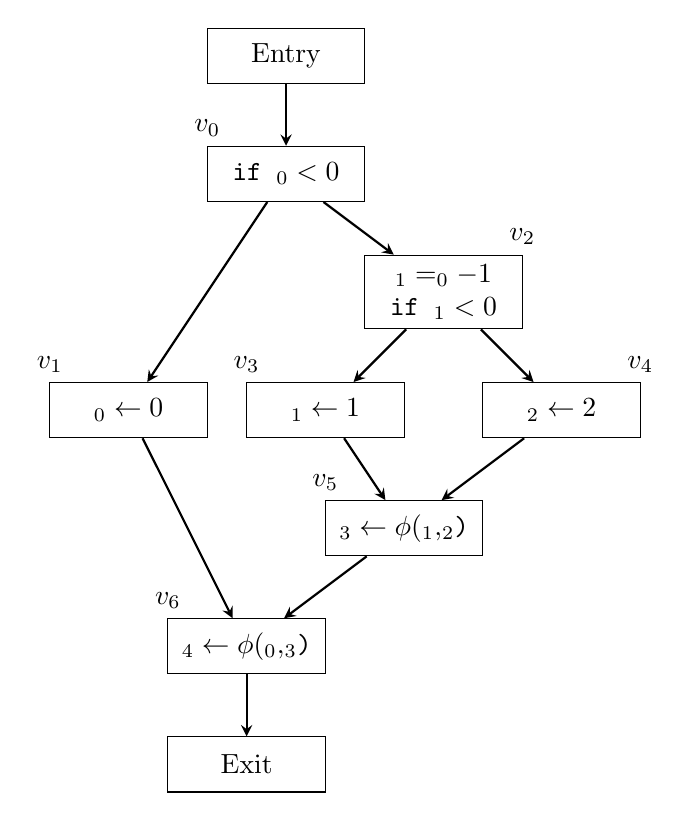
\begin{tikzpicture}
                \tikzstyle{node} = [rectangle, minimum width=2cm, minimum height=.7cm, text centered, draw=black, node distance=1.5cm]
                \tikzstyle{arrow} = [thick,->,>=stealth]
                
                \node (entry) [node] {Entry};
                \node (b1) [node, below of=entry, align=center, label={[xshift=-1cm]$v_0$}] {\texttt{if $\mIn_0 < 0$}};
                \node (b2) [node, below of=b1, xshift=-2cm, yshift=-1.5cm, label={[xshift=-1cm]$v_1$}] {\texttt{$\mOut_0 \leftarrow 0$}};
                
                \node (b3) [node, below of=b1, xshift=+2cm, align = center, label={[xshift=+1cm]$v_2$}] {$\mIn_1 = \mIn_0 - 1$\\\texttt{if $\mIn_1 < 0$}};
                
                \node (b4) [node, below of=b3, xshift=-1.5cm, label={[xshift=-1cm]$v_3$}] {\texttt{$\mOut_1 \leftarrow 1$}};
                \node (b5) [node, below of=b3, xshift=+1.5cm, label={[xshift=+1cm]$v_4$}] {\texttt{$\mOut_2 \leftarrow 2$}};
                \node (b6) [node, below of=b5, xshift=-2cm, label={[xshift=-1cm]$v_5$}] {\texttt{$\mOut_3 \leftarrow
                \phi(\mOut_1, \mOut_2$)}};
                
                \node (b7) [node, below of=b6, xshift=-2cm, label={[xshift=-1cm]$v_6$}] {\texttt{$\mOut_4 \leftarrow
                \phi(\mOut_0, \mOut_3$)}};
                \node (exit) [node, below of=b7] {Exit};

                \draw [arrow] (entry) -- (b1);
                \draw [arrow] (b1) -- (b2);
                \draw [arrow] (b1) -- (b3);
                \draw [arrow] (b2) -- (b7);
                \draw [arrow] (b3) -- (b4);
                \draw [arrow] (b3) -- (b5);
                \draw [arrow] (b4) -- (b6);
                \draw [arrow] (b5) -- (b6);
                \draw [arrow] (b6) -- (b7);
                \draw [arrow] (b7) -- (exit);
            \end{tikzpicture}
    \end{minipage}\hfill
    \caption{Program text and CFG of a short example program}
    \label{fig:doubleIf}
\end{figure}

In a CFG, the edges represent the jumps between basic blocks. We define the edge condition function $follow: \mbb_p \to \mbform$ to annotate CFG edges with propositional formulas, that evaluate to true iff the jump between the two incident basic blocks is taken during an execution.


% might need this later somewhere, not sure
%\begin{definition}[Jump Expression]
 %   For each basic block $b \in \mbb_p$, we define $jump(b)$ as the program expression that decides which successor block of $b$ will be executed.
 %   \begin{center}
 %       $jump: \: \mbb_p \to \mathtt{Expr}$
 %   \end{center}
 %   If $b$ ends in a conditional jump, $jump(b)$ is the expression of the conditional jump instruction.
    
 %   If $b$ ends in an unconditional jump or $b$ is the \texttt{exit} block, we define $b$ as the constant expression \ttt.
%\end{definition}

%\begin{definition}[Edge Condition]
%    Let $CFG(p) = (\mbb_p, E)$ be the CFG of the program $p$.We define
%    \begin{center}
%        $follow: E \to \mbform$\\
%        $(b_0, b_1) \mapsto 
%        \begin{cases}
%            \mathcal{E}(jump(b_0)) & \text{if the execution follows $e$ for $jump(b_0) = \mttt$}\\
%            \lnot \mathcal{E}(jump(b_0)) & \text{if the execution follows $e$ for $jump(b_0) = \mfff$}
%        \end{cases}$
%    \end{center}
%    For every edge $e := (b_0, b_1) \in E$, the propositional formula $follow(e)$ is true iff the control flow during an execution of $p$ jumps from $b_0$ to $b_1$.
%\end{definition}

Figure \ref{ex:ec} shows the CFG of the example program \ref{fig:doubleIf} with edges being annotated with their edge conditions.

\begin{figure}
    \centering
                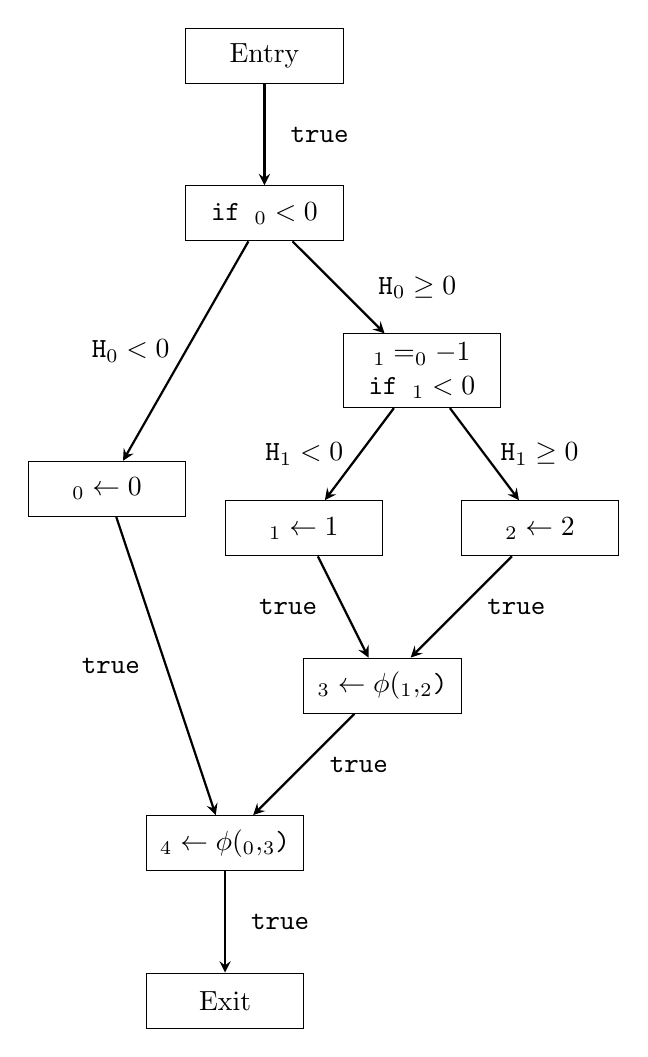
\begin{tikzpicture}
                \tikzstyle{node} = [rectangle, minimum width=2cm, minimum height=.7cm, text centered, draw=black, node distance=2cm]
                \tikzstyle{arrow} = [thick,->,>=stealth]
                
                \node (entry) [node] {Entry};
                \node (b1) [node, below of=entry, align=center] {\texttt{if $\mIn_0 < 0$}};
                \node (b2) [node, below of=b1, xshift=-2cm, yshift=-1.5cm] {\texttt{$\mOut_0 \leftarrow 0$}};
                
                \node (b3) [node, below of=b1, xshift=+2cm, align = center] {$\mIn_1 = \mIn_0 - 1$\\\texttt{if $\mIn_1 < 0$}};
                
                \node (b4) [node, below of=b3, xshift=-1.5cm] {\texttt{$\mOut_1 \leftarrow 1$}};
                \node (b5) [node, below of=b3, xshift=+1.5cm] {\texttt{$\mOut_2 \leftarrow 2$}};
                \node (b6) [node, below of=b5, xshift=-2cm] {\texttt{$\mOut_3 \leftarrow
                \phi(\mOut_1, \mOut_2$)}};
                
                \node (b7) [node, below of=b6, xshift=-2cm] {\texttt{$\mOut_4 \leftarrow
                \phi(\mOut_0, \mOut_3$)}};
                \node (exit) [node, below of=b7] {Exit};

                \draw [arrow] (entry) -- (b1) node[midway, xshift=.7cm] {\texttt{true}};
                \draw [arrow] (b1) -- (b2) node[midway, xshift=-.7cm] {$\mathtt{H}_0 < 0$};
                \draw [arrow] (b1) -- (b3) node[midway, xshift=1cm] {$\mathtt{H}_0 \geq 0$};
                \draw [arrow] (b2) -- (b7) node[midway, xshift=-.7cm] {\texttt{true}};
                \draw [arrow] (b3) -- (b4) node[midway, xshift=-.7cm] {$\mathtt{H}_1 < 0$};
                \draw [arrow] (b3) -- (b5) node[midway, xshift=.7cm] {$\mathtt{H}_1 \geq 0$};
                \draw [arrow] (b4) -- (b6) node[midway, xshift=-.7cm] {\texttt{true}};
                \draw [arrow] (b5) -- (b6) node[midway, xshift=.7cm] {\texttt{true}};
                \draw [arrow] (b6) -- (b7) node[midway, xshift=.7cm] {\texttt{true}};
                \draw [arrow] (b7) -- (exit) node[midway, xshift=.7cm] {\texttt{true}};
            \end{tikzpicture}
    \caption{CFG from figure \ref{ex:ec} with annotated edges. The annotations represent the formulas $follow(e)$. For easier reading the formulas are given as propositional formulas with linear integer arithmetic instead of bit vector logic.}
    \label{ex:ec}
\end{figure}

\paragraph{Execution Conditions for Basic Blocks}
A basic block $b$ in a program is executed, if one of its predecessor blocks is executed and if the condition for execution to jump from said predecessor to the block $b$ is fulfilled. A special case is a program's entry block, which is executed in every run. This leads to the following definition: 

\begin{definition}[Execution Condition]
    For every basic block $b \in \mbb_p$, its \emph{execution condition} is a propositional formula $f_b$, where $\mathcal{V}_\mIn(f_b) = \mttt \iff \text{basic block $b$ is executed in a program run with inputs \In}$. \td{put this in lemma?}
    \begin{center}
        $exec: \mbb_p \to \mbform$\\
        \begin{align*}
            exec(b) &:= \begin{cases}
                \mttt &  b = \mathtt{entry}\\
                \bigvee\limits_{p \in pred(b)} follow((p, b)) \land exec(p) & \text{otherwise}\\
        \end{cases}\\
        \end{align*}
    \end{center}
\end{definition}

\paragraph{Example Computation}
Table \ref{tab:exec} shows the execution conditions of all the basic blocks of example \ref{fig:doubleIf}. We show how these results were computed in detail for blocks $v_3$ and $v_5$:
\begin{itemize}
    \item Basic block $v_3$ has one predecessor $v_2$ with $exec(v_2) = \mIn_0 \geq 0$. The edge $(v_2, v_3)$ represents a conditional jump that is taken iff the condition $follow((v_2, v_3)) := \mIn_1 < 0$ is fulfilled.
    \begin{align*}
        exec(v_3) &:= follow((v_2, v_3)) \land exec(v_2) \\
        &= \mIn_0 \geq 0 \land \mIn_1 < 0 \\
    \end{align*}
    
    \item Basic block $v_5$ has two predecessors $v_3$ and $v_4$. Their execution conditions are given in table \ref{tab:exec}. Both incoming edges of $v_5$ represent unconditional jumps, thus their edge conditions evaluate to $\mttt$.
    \begin{alignat*}{2}
        exec(v_5) \quad &:= follow((v_3, v_5)) \land exec(v_3) \quad &\lor & \quad follow((v_4, v_5)) \land exec(v_4)\\
        &= \mttt \land (\mIn_0 \geq 0 \land \mIn_1 < 0) &\lor & \quad \mttt \land (\mIn_0 \geq 0 \land \mIn_1 \geq 0)\\
        &= \mIn_0 \geq 0 \land (\mIn_1 < 0 \lor \mIn_1 \geq 0) \\
        &= \mIn_0 \geq 0
    \end{alignat*}
\end{itemize}

\begin{figure}
    \centering
    \begin{tabular}{ |c|c| } 
        \hline
        $b$ & $exec(b)$ \\
        \hline
        $\mathtt{entry}$ & $\mttt$ \\
        $v_0$ & $\mttt$ \\
        $v_1$ & $\mathtt{H}_0 < 0$ \\
        $v_2$ & $\mathtt{H}_0 \geq 0$ \\
        $v_3$ & $\mathtt{H}_0 \geq 0 \land \mathtt{H}_1 < 0$ \\
        $v_4$ & $\mathtt{H}_0 \geq 0 \land \mathtt{H}_1 \geq 0$ \\
        $v_5$ & $\mathtt{H}_0 \geq 0$ \\
        $v_6$ & $\mttt$ \\
        $\mathtt{exit}$ & $\mttt$ \\
        \hline
    \end{tabular}
    \caption{Evaluation of $exec(\cdot)$ for the basic blocks of program \ref{fig:doubleIf}}
    \label{tab:exec}
\end{figure}

\paragraph{Combining Implicit and Explicit Information Flows in $\phi$-functions}
The execution conditions introduced in the previous section can be used to evaluate which basic blocks will be executed depending on the inputs. They contain all control flow dependencies that are present in the program.

The implicit and explicit information flows, that so far we have analysed separately, are combined when a value is assigned the result of a $\phi$-function. Let the value $v_0$ be defined via $v_0 := \phi(v_1, v_2), \: v_1, v_2 \in \val_p$ and $e$ is part of basic block $b_0$ with predecessors $\{b_1, b_2\}$. The situation is shown in figure \ref{fig:phi}.

To evaluate the $\phi$-expression and compute the dependency vector for value $v_0$, we use the following defined in \ref{fig:exprPhi}.

\begin{definition}[Ternary Operator]
    We define the ternary operator $\mathbb{IF}(\cdot, \cdot, \cdot)$ as:
    \begin{center}
        $\mathbb{IF}: \mbform \times \mbform \times \mbform \to \mbform$\\
        $\mathbb{IF}(c, x, y) := (c \implies x) \land (\lnot c \implies y)$
    \end{center}
    We canonically extend the definition to include propositional vectors:
    \begin{center}
        $\mathbb{IF}: \mbform \times \mbform^k \times \mbform^k \to \mbform^k$\\
        $\mathbb{IF}(c, x, y) := [\mathbb{IF}(c, x^i, y^i)]_{i = 0}^k$
    \end{center}
\end{definition}

The correctness of this definition follows from the following considerations:

If we compute the dependency vector $dVec(v_0) := \mathcal{E}(\phi(v_1, v_2)$ of the value $v_0$, we can assume that the basic block $def(v_0) = b_0$ is executed. Otherwise, any assignment to $v_0$ and the information contained in the assignment is irrelevant for the leakage analysis of the execution in question.

If the basic block $b_0$ is executed, at least one of its predecessors $b_1, \: b_2$ must have been executed as well for the execution to reach $b_0$. Furthermore it is impossible for both of $b_0$'s predecessors to have been executed, since so far we only consider loop-free programs, that have no back-edges in their CFG. It follows that the condition $exec(b_1) \veebar exec(b_2)$ must hold for any input value. It is therefore sufficient to only check the execution condition of $b_1$ in the definition of $\mathcal{E}(\phi(v_1, v_2))$.

\begin{figure}
\begin{subfigure}[t]{.4\textwidth}
    \centering
    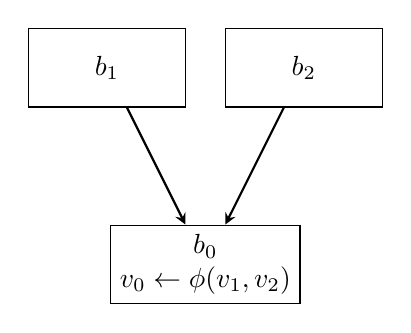
\begin{tikzpicture}
        \tikzstyle{node} = [rectangle, minimum width=2cm, minimum height=1cm, text centered, draw=black, node distance=2.5cm]
        \tikzstyle{arrow} = [thick,->,>=stealth]
                
                \node (b1) [node] {$b_1$};
                \node (b2) [node, right of=b1] {$b_2$};
                \node (b0) [node, below of=b1, xshift=1.25cm, align=center] {$b_0$ \\ $v_0 \leftarrow \phi(v_1, v_2)$};
                
                \draw[arrow] (b1) -- (b0);
                \draw[arrow] (b2) -- (b0);
                
    \end{tikzpicture}
    \caption{Section of a CFG that contains a $\phi$-function.}
    \label{fig:phi}
\end{subfigure}
\hfill
\begin{subfigure}[t]{.5\textwidth}
    \begin{equation*}
\mathcal{E}(\phi(v_1, v_2)) := \mathbb{IF}(exec(b_1), v_1, v_2)
\end{equation*}
\caption{Extension of the definition of $\mathcal{E}(\cdot)$ in \ref{fig:expr} for the evaluation of $\phi$-functions.}\label{fig:exprPhi}
\end{subfigure}
\caption{Handling of $\phi$-functions during the dependency analysis}
\end{figure}

\paragraph{Example (cont'd)}
Combining the analysis elements from section \ref{sec:design}, we can complete the dependency analysis of the example program \ref{fig:doubleIf}. The algorithm for the dependency analysis of loop-free, call-free programs is shown in \ref{alg:depAna}. The algorithm returns the dependency vector of the leaked value.

Figure \ref{fig:exFinished} shows the dependency vectors of all program values. The analysis of the example program returns the vector
\begin{align*}
    dVec(\mOut_4) &= \mathbb{IF}(\mIn_0 < 0, dVec(\mOut_0), dVec(\mOut_3)) \\
    &= \mathbb{IF}(\mIn_0 < 0, 0, \mathbb{IF}(\mIn_0 \geq 0 \land (\mIn_0 - 1) < 0, dVec(\mOut_1), dVec(\mOut_2))) \\
    &= \mathbb{IF}(\mIn_0 < 0, 0, \mathbb{IF}(\mIn_0 \geq 0 \land (\mIn_0 - 1) < 0, 1, 2))
\end{align*}

If we substitute the variable $\mIn_0$ in $dVec(\mOut_4)$ for a concrete input value, $dVec(\mOut_4)$ will evaluate to the output value $\mOut_4$ of the execution.

\begin{algorithm}
        \hspace*{\algorithmicindent} \textbf{Input} $CFG(p) = (\mbb_p, \: E):$ CFG of input program $p$ in SSA form.\\ 
        \hspace*{\algorithmicindent} \hspace*{\algorithmicindent} $p$ takes a secret input $\mIn$ and leaks a public output value $\mOut$. \\
        \hspace*{\algorithmicindent} \textbf{Output} $leaked: \mbform^w$\\
        \begin{algorithmic}[1]
            \State $blocks: (\mbb_p \to \mbform)$
            \State $dVec: (\val_p \to \mbform^w)$
            
            \For{$b \in \mbb_p$ in topological order}
                \State $blocks(b) \leftarrow exec(b)$
                \For{$v \leftarrow e \in Statements(b)$}
                    \State $dVec(v) \leftarrow \mathcal{E}(e)$
                \EndFor
            \EndFor
            \State $leaked \leftarrow dVec(\mOut)$
    \end{algorithmic} 
    \caption{Dependeny Analysis}\label{alg:depAna}
\end{algorithm}

\begin{figure}
    \centering
    \begin{tikzpicture}
                \tikzstyle{node} = [rectangle, minimum width=2cm, minimum height=.7cm, text centered, draw=black, node distance=3cm]
                \tikzstyle{arrow} = [thick,->,>=stealth]
                
                \node (entry) [node] {Entry};
                \node (b1) [node, below of=entry, align=center, label={[xshift=-1cm]$v_0$}] {\texttt{if $\mIn_0 < 0$}};
                \node (b2) [node, below of=b1, xshift=-2cm, yshift=-1.5cm, label={[xshift=-1cm]$v_1$}] {\texttt{$\mOut_0 \leftarrow 0 \quad \color{blue}{dVec(\mOut_0) = 0}$}};
                
                \node (b3) [node, below of=b1, xshift=+5cm, align = center, label={[xshift=+1cm]$v_2$}] {$\mIn_1 = \mIn_0 - 1 \quad \color{blue}{dVec(\mIn_1) = H_0 - 1}$\\\texttt{if $\mIn_1 < 0$}};
                
                \node (b4) [node, below of=b3, xshift=-2.5cm, label={[xshift=-1cm]$v_3$}] {\texttt{$\mOut_1 \leftarrow 1 \quad \color{blue}{dVec(\mOut_1) = 1}$}};
                \node (b5) [node, below of=b3, xshift=+2.5cm, label={[xshift=+1cm]$v_4$}] {\texttt{$\mOut_2 \leftarrow 2 \quad \color{blue}{dVec(\mOut_2) = 2}$}};
                \node (b6) [node, below of=b5, xshift=-2.5cm, label={[xshift=-1cm]$v_5$}, align=center] {$\mOut_3 \leftarrow
                \phi(\mOut_1, \mOut_2)$\\$ \color{blue}{dVec(\mOut_3) = \mathbb{IF}(\mIn_0 \geq 0 \land (\mIn_0 - 1) < 0, dVec(\mOut_1), dVec(\mOut_2)) }$};
                
                \node (b7) [node, below of=b6, xshift=-5cm, label={[xshift=-1cm]$v_6$}, align=center] {$\mOut_4 \leftarrow
                \phi(\mOut_0, \mOut_3 )$\\$\color{blue}{dVec(\mOut_4) = \mathbb{IF}(\mIn_0 < 0, dVec(\mOut_0), dVec(\mOut_3)) }$};
                \node (exit) [node, below of=b7] {Exit};

                \draw [arrow] (entry) -- (b1);
                \draw [arrow] (b1) -- (b2);
                \draw [arrow] (b1) -- (b3);
                \draw [arrow] (b2) -- (b7);
                \draw [arrow] (b3) -- (b4);
                \draw [arrow] (b3) -- (b5);
                \draw [arrow] (b4) -- (b6);
                \draw [arrow] (b5) -- (b6);
                \draw [arrow] (b6) -- (b7);
                \draw [arrow] (b7) -- (exit);
            \end{tikzpicture}
    \caption{CFG of program \ref{fig:doubleIf} annotated with the dependency vectors of each program value}
    \label{fig:exFinished}
\end{figure}
